%!TEX root=../../../main.tex

In order to disseminate annotation data in a standardised manner two issues
need to be handled:
\begin{enumerate}
  \item Format annotation using an established specification.
  \item Provide an easy to use mechanism for data access.
\end{enumerate}

Regarding the data format, we have chosen the Open Annotation data model, which
recommends using a JSON-LD RDF serialisation for making annotations public
\cite{ref:oa}. Basically, the specification provides a context, in which the
keys are the various OA model components, and the values IRI to various
ontologies, such as FOAF, Dublin Core Metadata Element Set, RDF or the specific
OA one.

This context can be used by applications to convert their own internal
representations to a standard JSON-LD document; if the internal model is
already in JSON form, this can be achieved directly by compaction.

Despite employing a JSON model in our implementation, we have chosen to
programmatically apply the processing steps. Namely, a thin interface over
JSONAlchemy was implemented\footnote{The code for this wrapper is already
included in the source tree of the next Invenio version and will be shipped
separately of the annotation features.}, allowing objects stored in JSON form
to specify their custom translation method. This method has a default context
specified, but custom ones can also be supplied, given that the object class
has the required flexibility.

For the annotations, the method will use the OA context and apply a number of
simple conversions. Let us consider the targeted annotations use-case,
described in Section \ref{sec:notes}, for which the conversions are as follows:
\begin{itemize}
  \item The main identifier of the resource is a IRI pointing to a endpoint of
        the Invenio installation which can supply annotations in the internal
        JSON format; this should not be usually used, but is included for
        completeness. The type of the resource is \texttt{Annotation} in the
        OA vocabulary.
  \item The OA \texttt{annotatedBy} field is filled with information regarding
        the user that created the annotation. Recall that, internally, we store
        only an identifier, which can be used to retrieve all other associated
        information, such as the name and email address. If, instead of applying
        the explicit conversion process, the JSON-LD compaction routine would be
        used, the mentioned information would need to be directly included in
        the annotation JSON model, resulting in information duplication. Another
        solution would be to provide only minimal information regarding users,
        namely an IRI where more information could be retrieved from.
  \item For the \texttt{annotatedAt} field, the time stamp is provided as-is. A
        note here is that, as data producers have no knowledge regarding their
        consumers, time zone information, usually as a value denoting the offset
        from the Coordinated Universal Time (UTC) needs to be included.
  \item For the \texttt{hasBody} field, the annotation content is provided, along
        with its format (\texttt{format/plain}) and encoding (Universal
        Transformation Formats (UTF))
  \item For the \texttt{hasBody} field, the annotation content is provided, along
        with its format (\texttt{format/plain}) and encoding (Universal
        Transformation Formats (UTF)).
  \item The \texttt{hasTarget} field is encoded as the IRI to the record of the
        document being annotated, along with a OA \texttt{FragmentSelector}
        data type, which specifies to what part of the document the annotation
        refers to (a marker such as \textit{``second paragraph on third page''},
        encoded in the manner described in Section \ref{sec:notes}). Note that
        if a method of accessing document fragments directly through a valid
        IRI is provided, specifying the selector is no longer necessary.
\end{itemize}
For annotations on Invenio Web pages the process is similar, except for the
target field, which can be identified uniquely by an IRI. An example of a
compacted JSON-LD representation of document annotation is included in Fig.
\ref{lst:annojson}.

\begin{figure}[!ht]
  \centering
  \fbox{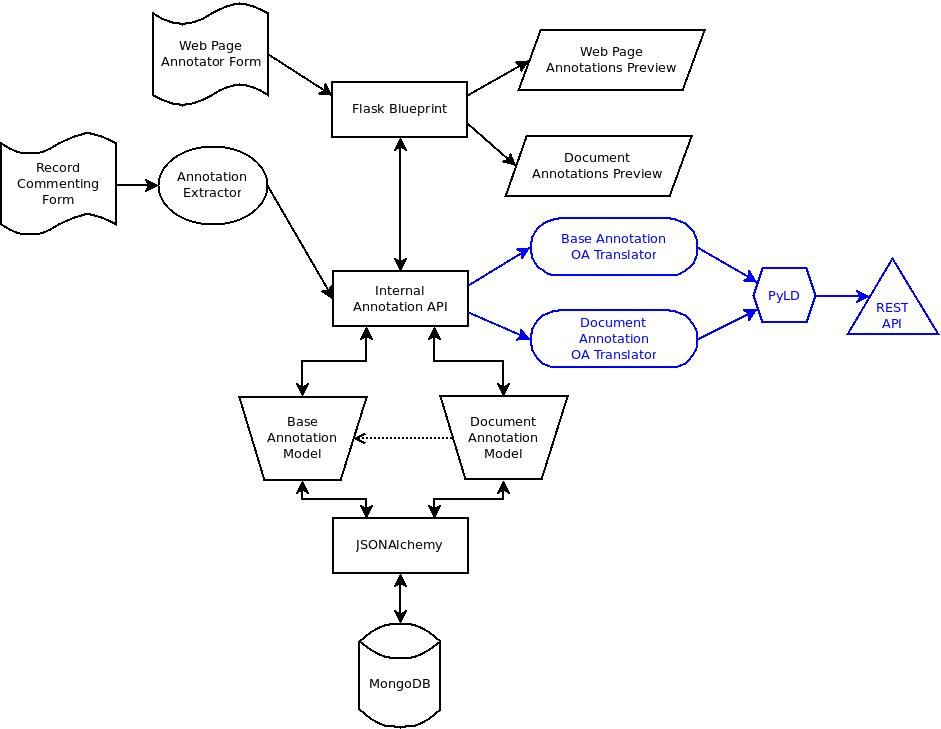
\includegraphics[scale=0.5]{static/dia/rest_anno.jpeg}}
  \caption[Annotation dissemination workflow]
          {Annotation dissemination workflow; after being translated to a proper
           standardised format (Open Annotation JSON-LD) and processed by PyLD,
           annotations can be served by the Invenio REST API to concerned
           third-parties.}
  \label{fig:restanno}
\end{figure}

FIXME: REST, add annos by REST
